\documentclass[runningheads]{llncs}

% ---------- packages ----------
\usepackage{amsmath,amssymb}
\usepackage{graphicx}
\usepackage{booktabs}
\usepackage{array}
\usepackage{xcolor}
\usepackage{tikz}
\usetikzlibrary{arrows.meta,positioning,shapes.geometric,calc}
\usepackage{url}
\usepackage[hidelinks]{hyperref}

% ---------- tikz styles ----------
\tikzset{
  box/.style={rectangle, rounded corners=2pt, draw=black!70, fill=blue!6,
    align=center, minimum height=8mm, inner sep=4pt, font=\small},
  db/.style={cylinder, shape border rotate=90, aspect=0.25, draw=black!70,
    fill=orange!12, align=center, minimum height=10mm, font=\small},
  llm/.style={rectangle, rounded corners=2pt, draw=black!70, fill=green!8,
    align=center, minimum height=8mm, inner sep=4pt, font=\small},
  flow/.style={-{Stealth[length=2mm]}, draw=black!70},
  step/.style={rectangle, rounded corners=2pt, draw=black!70, fill=gray!8,
    align=center, minimum height=7mm, text width=24mm, inner sep=3pt, font=\footnotesize},
  gnode/.style={rectangle, rounded corners=2pt, draw=black!70, fill=blue!6,
    align=center, minimum height=7mm, text width=22mm, inner sep=3pt, font=\footnotesize}
}

\begin{document}

\title{HospitAI: Combining Mixed-Data Patient Clustering, Clinical Sequence Mining and AI-Generated Interpretation in a Hospital Analytics Platform}
\titlerunning{HospitAI: Clustering, Sequence Mining and AI Interpretation}

\author{Author Name\inst{1}}
\authorrunning{Author Name}
\institute{Faculty of Computer Science, University Name, City, Country\\
\email{author@email.example}}

\maketitle

\begin{abstract}
Hospitals store large amounts of electronic health record (EHR) data, but this data is rarely turned into a clear view of patient groups and their care over time. We present HospitAI, a platform that joins three analytics steps in one tool. It first groups patients with K-Prototypes, a clustering method for mixed numerical and categorical data. It then mines frequent clinical sequences with a pipeline built around PrefixSpan and adapted to the medical domain. Finally, it uses a large language model to turn the computed statistics into short summaries for both clinicians and patients. The main technical part is the sequence-mining pipeline. Rather than ranking patterns only by frequency, we score them with a geometric mean lift measure and apply diversity filters, so the output favours meaningful care paths over frequent but trivial ones. We also mine each patient cluster separately and treat statistical outliers as a distinct group, which makes rare but important pathways such as oncology, dialysis and heart failure visible. On a synthetic dataset of about 22{,}000 patients we obtain four stable clusters and per-cluster pattern sets that match recognisable care populations.

\keywords{Hospital analytics \and Patient clustering \and K-Prototypes \and Sequential pattern mining \and PrefixSpan \and Large language models \and Electronic health records.}
\end{abstract}

% !TEX root = ./main.tex

\section{Introduction}

Modern hospitals store very large amounts of data in their electronic health record (EHR) systems. Every encounter leaves a trace, including diagnoses, prescribed medications, procedures and care plans. This data could help hospital managers and clinicians understand who their patients are and how care really happens. In practice most of it stays unused, because the tables are large, noisy and hard to read without technical skills.

Three difficulties stand in the way. The first one is patient heterogeneity. A young person with a single fracture and an older patient with diabetes, hypertension and kidney failure should not be analysed as if they were the same, yet a global average over all patients hides this variety. The second difficulty is the temporal nature of care. Treatment is not a single snapshot but a sequence of events that develops over months or years, and the order of those events often carries the clinical meaning. The third difficulty is communication. Even a correct model usually produces a list of numbers or codes that a clinician or a patient cannot interpret quickly.

This paper presents HospitAI, a web platform that tackles these three difficulties together. It was developed as part of an undergraduate thesis. The platform connects a clustering step, a sequence-mining step and a language step, so the same patient data can be examined from several angles inside one tool.

For patient heterogeneity we use K-Prototypes \cite{huang1998kprototypes}, a clustering method designed for mixed data, because clinical features are partly numerical (age, number of medications) and partly categorical (gender, main care plan). For the temporal aspect we build a sequence-mining pipeline on top of PrefixSpan \cite{pei2004prefixspan} and adapt it to clinical data, so that it returns useful care paths instead of obvious repetitions. For communication we add a large language model (LLM) that reads the precomputed statistics and writes short summaries in plain language for two audiences, the medical staff and the patient.

Our contributions are the following:

\begin{itemize}
  \item An integrated and working platform that combines mixed-data patient clustering, clinical sequence mining and AI-generated interpretation, with a clean separation between the offline analytics and the web application that serves the results.
  \item A feature-engineering process that turns several raw EHR tables into a compact set of patient features, with explicit handling of skewed counts, missing vital signs and statistical outliers.
  \item A domain-adapted sequence-mining pipeline around PrefixSpan that ranks patterns with a geometric mean lift score and a set of diversity rules. This strongly reduces trivial output and keeps clinically meaningful care paths near the top.
  \item A controlled use of an LLM as a ``verbaliser'' over fixed statistics, together with a guarded natural-language-to-SQL agent, so that non-technical users can both read and query the data.
\end{itemize}

The paper is organised as follows. Section~\ref{sec:related} reviews related work. Section~\ref{sec:system} describes the system architecture and the data. Sections~\ref{sec:clustering},~\ref{sec:mining} and~\ref{sec:ai} explain the clustering, the sequence mining and the AI interpretation. Section~\ref{sec:results} reports the results, and Section~\ref{sec:conclusion} discusses limitations and future work.

% !TEX root = ./main.tex

\section{Related Work}
\label{sec:related}

Learning patient groups and care paths from health data is an active research area, and our work builds on several lines of it.

\paragraph{Surveys of patient-pathway analysis.}
Two recent reviews map the field well. Rosa et al. \cite{rosa2022modelling} survey how patient pathways are modelled and mined, and they separate sequence-mining approaches from process-mining approaches. Flothow et al. \cite{flothow2023} review the analytical methods used to identify sequences of healthcare utilisation, and they report a useful split: clustering is mostly used to describe full care trajectories, while pattern-mining methods are mostly used to identify shorter subsequences. HospitAI sits between these two groups, because we cluster patients first and then mine sequences inside each cluster.

\paragraph{Combining clustering and sequence mining.}
The work closest to ours mixes the two ideas. Najjar et al. \cite{najjar2018twostep} propose a two-step method that first clusters individual medical visits with K-Prototypes and then builds higher-level treatment pathways. This is a strong precedent, because it relies on the same mixed-data clustering algorithm that we use. Baudrier et al. \cite{baudrier2022} combine a sequential pattern-mining algorithm with care-trajectory clustering on kidney cancer patients, and they show that the resulting groups differ in real outcomes such as mortality. Vogt et al. \cite{vogt2017} apply sequence clustering to ambulatory care pathways in insurance claims and find typical care patterns for heart-failure patients. Our design follows the same spirit but reverses the order: clustering comes first and defines the scope, and mining then runs inside each scope.

\paragraph{Sequence mining from EMR with interpretation.}
Perer et al. \cite{perer2015mining} mine frequent event sequences from electronic medical records and connect them to patient outcomes, with a strong focus on visual exploration. Their system shows that frequent sequences can recover care patterns that are clinically meaningful, and sometimes even unknown to the treating physician. This motivates our own attention to pattern quality, because raw frequency on its own is not enough.

\paragraph{Clustering of patients on EHR data.}
Several works study how to group patients well. Yang et al. \cite{yang2024} build a smart-healthcare system that clusters patients on mixed medical data, including text embeddings, and compare several clustering methods. Aljohani \cite{aljohani2024} compares eight clustering algorithms for patient stratification on EHR data and ranks them with a multi-criteria decision framework. These works confirm that clustering is a useful tool for patient stratification, and that the choice of algorithm and evaluation metric has a large impact.

\paragraph{Process mining as an alternative.}
A different family of methods discovers care processes from event logs. Murazzano et al. \cite{murazzano2026} apply process mining to chronic respiratory patients and find high variability in their clinical pathways. We mention this line of work because it targets the same goal as our sequence mining, namely understanding how care actually happens, but with a different technique.

In summary, clustering and sequence mining are both well studied in healthcare, and a few works already combine them. What is still missing is a single, practical tool that connects cluster-scoped mining, a pattern ranking made for clinical usefulness, and an automatic interpretation layer that non-experts can read. HospitAI is our attempt to close that gap.

\section{System Architecture and Data}
\label{sec:system}

\subsection{Architecture}

HospitAI is divided into a web application and an offline analytics part. The web side has a frontend built with Next.js and a backend built with FastAPI. The backend follows a strict layered structure: API routers call a service layer, the service layer calls a repository layer, and only the repository layer talks to the database. This separation keeps the database queries in one place and makes the code easier to maintain. All persistent data lives in a single PostgreSQL database. Figure~\ref{fig:arch} shows the main components.

The two heavy machine-learning steps, clustering and sequence mining, do not run inside a web request. They are separate Python scripts that we run offline, because they are slow and only need to run when the data changes. Each script reads from the database, computes its result and writes it back into dedicated tables. The web application then only reads these tables, which keeps the user interface responsive. A single LLM, accessed through the OpenAI API, is used for every text-generation task in the platform.

\begin{figure}[t]
\centering
\begin{tikzpicture}[node distance=6mm and 9mm]
  \node[box, fill=blue!8] (fe) {Frontend (Next.js + Redux)};
  \node[box, below=of fe] (api) {Backend API (FastAPI routers)};
  \node[box, below=of api] (svc) {Service layer};
  \node[box, below=of svc] (repo) {Repository layer};
  \node[db, below=9mm of repo] (db) {PostgreSQL};
  \node[step, right=16mm of svc, text width=26mm] (ml) {Offline ML scripts:\\K-Prototypes\\PrefixSpan};
  \node[llm, left=12mm of svc, text width=20mm] (llm) {LLM\\(OpenAI GPT)};

  \draw[flow] (fe) -- (api);
  \draw[flow] (api) -- (svc);
  \draw[flow] (svc) -- (repo);
  \draw[flow] (repo) -- (db);
  \draw[flow] (svc) -- (llm);
  \draw[{Stealth[length=2mm]}-{Stealth[length=2mm]}, draw=black!70] (ml) |- (db)
       node[pos=0.28,right,font=\footnotesize]{read / write};
\end{tikzpicture}
\caption{High-level architecture. The web application reads precomputed results, while the clustering and mining scripts run offline and write their output into the database.}
\label{fig:arch}
\end{figure}

\subsection{Data}

For development and experiments we use a synthetic dataset generated with Synthea, an open-source patient simulator. Synthetic data is a sensible choice for a student project, because it removes privacy and legal barriers while keeping a realistic clinical structure. The dataset contains about 22{,}284 patients, with the usual clinical tables: encounters, conditions, medications, procedures, observations and care plans. A loading script reduces the data to a single hospital and a fixed set of providers, cleans the dates, and computes helper fields such as patient age and treatment duration.

The dataset is large enough to make the analytics non-trivial. The event tables used for sequence mining hold roughly 727{,}000 conditions, 913{,}000 medications, 3.2 million procedures and 70{,}000 care plans, which together give close to five million clinical events. After cleaning, the vocabulary of distinct event items is around 1{,}170.

The same database stores both the raw clinical tables and the analytics output. Clustering writes one row per patient with the cluster label, a flag for outliers, a two-dimensional projection for visualisation, and a cached set of features in a JSON column. Sequence mining writes the discovered patterns into one table and the patient-to-pattern membership into a link table. The interpretation step stores its generated text in JSON columns next to the cluster and pattern rows, so that each summary is computed only once and then reused.

% !TEX root = ./main.tex

\section{Patient Clustering}
\label{sec:clustering}

\subsection{Feature Engineering}

Clustering needs a clean table where each row is a patient and each column is a feature. Building this table is most of the effort, because the raw EHR data is spread over seven tables and is not ready for a model. We compute the features with SQL aggregation queries and then join them on the patient identifier.

We build a large pool of candidate features, around forty in total, and then keep a smaller subset for the final model. The candidates include encounter counts per type, disease flags derived by matching condition descriptions, counts of medications and procedures, averaged vital signs, and several derived indicators such as a readmission-risk tier and a preventive-to-reactive care ratio. We also compute a compact severity index by applying principal component analysis to a few log-transformed counts, which gives one number that summarises overall clinical load.

A few preprocessing choices deserve attention. Some counts are strongly right-skewed, so we apply a $\log(1+x)$ transform before scaling. The numerical features are then brought to a common range with min-max scaling. Vital signs such as blood pressure and glucose are often missing, so instead of filling them with the mean we put each value into a clinical bin and add an explicit ``Unknown'' bin. In this way the fact that a measurement is missing is kept as information, which is often itself meaningful. We do not one-hot encode the categorical features, because K-Prototypes works on them directly, and one-hot encoding would distort the mixed-distance balance.

The final configuration uses five numerical and eight categorical features, listed in Table~\ref{tab:features}.

\begin{table}[t]
\caption{Final feature set used by the clustering model.}
\label{tab:features}
\centering
\small
\begin{tabular}{@{}p{0.46\linewidth}p{0.46\linewidth}@{}}
\toprule
Numerical & Categorical \\
\midrule
age & gender \\
active conditions count & pregnancy history \\
total medications & has heart disease \\
total procedures & has diabetes \\
preventive-to-reactive ratio & has hypertension \\
 & condition burden (binned) \\
 & body-mass-index category \\
 & dominant care plan \\
\bottomrule
\end{tabular}
\end{table}

\subsection{The K-Prototypes Algorithm}

K-Prototypes \cite{huang1998kprototypes} extends K-Means to mixed data. For a patient $x$ with numerical attributes and categorical attributes, and a cluster prototype $c$, the distance is
\begin{equation}
d(x, c) \;=\; \sum_{j \in \text{num}} (x_j - c_j)^2 \;+\; \gamma \sum_{l \in \text{cat}} \delta(x_l, c_l),
\end{equation}
where $\delta(a,b)=0$ if $a=b$ and $1$ otherwise. The first term is the squared Euclidean distance on numerical features, and the second term counts the categorical mismatches. The weight $\gamma$ controls how much the categorical part contributes. The algorithm then minimises the total cost
\begin{equation}
J \;=\; \sum_{p=1}^{n} d\big(x_p, c_{a(p)}\big),
\end{equation}
where $a(p)$ is the cluster assigned to patient $p$. Like K-Means, it alternates between assigning each point to its nearest prototype and updating the prototypes, but the categorical part of the prototype is the most frequent value (the mode) rather than the mean.

We use the Huang initialisation. The weight $\gamma$ can be set by hand, but a common heuristic is to use the average spread (standard deviation) of the scaled numerical features, so that the two distance terms are on a comparable scale. In our final run we let the library choose $\gamma$ automatically, which gives a value near $0.084$.

Before fitting, we remove statistical outliers with a z-score rule on the most informative numerical features. We do not discard these patients. They receive the special cluster label $-1$ and are stored like every other patient. This is important for the next step, because these patients carry the high-acuity signal (cancer, dialysis, heart failure) that a balanced clustering tends to push aside.

\subsection{Evaluation and Model Selection}

Choosing the number of clusters and the feature set requires a metric that fits mixed data. The standard silhouette score and the Calinski-Harabasz and Davies-Bouldin indices all assume a Euclidean space. Applying them to one-hot encoded categories would over-emphasise the numerical spread and hide the categorical structure. For this reason our main metric is the silhouette computed on the Gower distance, which scales each numerical feature by its range and compares categorical values by agreement, in the same spirit as K-Prototypes. We use Calinski-Harabasz and Davies-Bouldin on a two-dimensional projection only as tie-breakers.

We also measure which features drive the partition. For numerical features we use the ANOVA effect size $\eta^2$, and for categorical features we use Cramer's V. Both give a value between zero and one that says how strongly a feature separates the clusters.

To pick a configuration we first look at an elbow plot of the clustering cost over a range of $k$, which suggests a small number of clusters. We then run a benchmark over 63 feature subsets and several hyperparameter values, and we rank the runs with a combined score that gives the largest weight to the Gower silhouette. The final rule is simple: we choose the smallest $k$ for which every cluster stays cohesive, because the clusters will be used as scopes for sequence mining and a weak cluster would produce weak patterns.

\section{Clinical Sequence Mining}
\label{sec:mining}

The second component studies the order of clinical events. Patients do not just have a set of diagnoses and treatments, they go through them in a certain order, and that order often holds the clinical meaning. We capture this with sequential pattern mining.

\subsection{Event Model and Preprocessing}

We define one sequence per patient, which is the patient's timeline of events sorted by date. Each event is tagged with a type prefix so that its source is always clear: \texttt{C} for a condition, \texttt{M} for a medication, \texttt{P} for a procedure and \texttt{CP} for a care plan. The same text in two different tables is treated as two different items, so a medication and a condition with similar names never collide. When several events happen on the same day, we order them in a fixed clinical order (condition, then medication, then procedure, then care plan), which makes the runs reproducible and follows the natural flow of care.

Real timelines are noisy, so we clean them before mining. We keep only the last two years of events per patient, because older events are less relevant to current care. We drop a short list of purely administrative items, such as routine ``medication review due'' entries, and a list of social-status findings that appear for almost everyone. We collapse immediate repetitions of the same item, which removes refill artefacts, and we cap each timeline at the last 25 events, which bounds the running time. Finally, each distinct item is mapped to an integer, because the mining engine works on integers.

\subsection{Mining and Scoring}

The mining engine is PrefixSpan \cite{pei2004prefixspan}, a classic algorithm that grows frequent patterns by repeatedly projecting the database on each discovered prefix. It avoids the candidate explosion of older methods, and it supports closed patterns, which drop a pattern when a longer pattern with the same support exists. We ask for closed patterns with a length between three and six and a minimum support of one percent of the patients. To get a good final set we mine a larger pool than we need, twenty times the target size, and then re-rank it, because the most frequent patterns are not always the most useful ones.

\begin{figure}[t]
\centering
\begin{tikzpicture}[node distance=4mm]
  \node[step] (a) {Raw events (C, M, P, CP)};
  \node[step, below=of a] (b) {Per-patient timelines};
  \node[step, below=of b] (c) {PrefixSpan (closed, length 3 to 6)};
  \node[step, below=of c] (d) {GML scoring + type bonus};
  \node[step, below=of d] (e) {Diversity selection};
  \node[step, below=of e] (f) {Top patterns per scope};
  \foreach \x/\y in {a/b,b/c,c/d,d/e,e/f} \draw[flow] (\x) -- (\y);
\end{tikzpicture}
\caption{The sequence-mining pipeline. PrefixSpan is the engine, but the scoring and diversity selection around it decide what the user finally sees.}
\label{fig:pipeline}
\end{figure}

The key idea is in the re-ranking, shown in Figure~\ref{fig:pipeline}. If we sort patterns by raw support, the top of the list is filled with frequent but useless chains, for example routine dental cleaning steps that almost every patient receives. To fix this we rank patterns with a geometric mean lift (GML) score. For a pattern $p$ made of $k$ items, with support $s(p)$ over $n$ patients and individual item supports $s(i)$, the score is
\begin{equation}
\mathrm{GML}(p) \;=\; \frac{s(p)/n}{\left(\displaystyle\prod_{i \in p} s(i)/n \right)^{1/k}} .
\label{eq:gml}
\end{equation}
This is the lift idea extended from two items to $k$ items through a geometric mean. The numerator is how often the whole chain occurs, and the denominator is the typical frequency of its single items. A pattern scores high when the full chain is more frequent than its parts would suggest, which is a sign that the steps really belong together. We compute Equation~\ref{eq:gml} in log space,
\begin{equation}
\log \mathrm{GML}(p) \;=\; \log s(p) - \log n - \frac{1}{k}\sum_{i \in p}\big(\log s(i) - \log n\big),
\end{equation}
which avoids numerical underflow when multiplying many small probabilities.

We then add a type-diversity bonus. The score is multiplied by $(1 + 0.3\,(t-1))$, where $t$ is the number of distinct event types in the pattern. This rewards a real care trajectory that mixes conditions, drugs and procedures over a pattern that merely repeats three medications.

\subsection{Diversity Selection}

A high score is not enough on its own, because the top of the list can still be full of near-duplicates. We therefore apply a selection stage with several rules. We drop patterns that contain three same-type events in a row, since these are usually within-step repetitions rather than trajectories. We run a second, global check for closed patterns, because re-ranking across branches can let dominated patterns slip through. We remove near-duplicates with a Jaccard test on the item sets, with a threshold of $0.80$. We also cap how many selected patterns may share the same first item or the same last item, which stops one common diagnosis from flooding the list.

Selection runs in two phases. In the first phase we reserve a small quota for full-spectrum patterns that contain all four event types, so that these rare but complete care paths are never crowded out. In the second phase we greedily fill the rest of the list under all the caps. At the end we sort the chosen set again by GML, so the order still reflects the ranking. Table~\ref{tab:params} lists the main parameters.

\begin{table}[t]
\caption{Main parameters of the sequence-mining pipeline.}
\label{tab:params}
\centering
\small
\begin{tabular}{@{}lll@{}}
\toprule
Parameter & Value & Meaning \\
\midrule
minimum support & 1\% & smallest pattern frequency \\
pattern length & 3 to 6 & items per pattern \\
recency window & 730 days & events kept per patient \\
events per patient & 25 & timeline length cap \\
over-mining factor & 20$\times$ & pool size before re-ranking \\
patterns kept & 500 & final patterns per scope \\
type-diversity weight & 0.3 & bonus per extra event type \\
Jaccard threshold & 0.80 & near-duplicate cut-off \\
per-prefix / per-suffix cap & 6 / 20 & shared first / last item \\
full-spectrum quota & 25 & reserved four-type patterns \\
\bottomrule
\end{tabular}
\end{table}

\subsection{Per-Cluster Scopes}

Finally, we run the whole pipeline once per scope. We mine the global cohort, and then we mine each cluster on its own, including the outlier group with label $-1$. After mining a cluster we remove the patterns that already appear in the global scope, so each cluster only shows what makes it distinctive. Each discovered pattern is stored together with the list of patients that contain it, computed with an inverted index over the rarest items first, which keeps the membership lookup fast.

\section{AI Interpretation}
\label{sec:ai}

The last component makes the analytics readable. We use a single LLM, but in a controlled way that keeps the text grounded in real numbers.

\subsection{The Verbaliser Principle}

The model never computes statistics by itself. Our code first computes everything, such as cluster averages, disease rates and the cohort statistics for a given pattern, and then passes these fixed numbers to the model with clear instructions to only describe them. We call this the verbaliser principle. Because the model receives the facts and is told not to invent or recompute anything, the risk of fabricated values is much lower than in a free-form prompt. The instructions also fix small style rules, for example the thresholds that count as high or low, so the wording stays consistent across patients.

The platform produces three kinds of text. For each cluster it writes a short card with a title, a colour, a one-line description, an insight and a recommendation. These cards are generated once, when the clustering is computed, and stored in the database. On demand, the platform writes a longer analysis of a single cluster or of a single mined pattern, returned as structured JSON. For a pattern the JSON contains a clinical interpretation, a plain-language summary for the patient, a list of risk signals and a list of recommendations. For a cluster it adds a risk level, key characteristics and suggested interventions, with each cluster value compared to the population average so the text can say whether a group is above or below the norm. All of these results are cached next to the cluster or pattern row, so the model is called only once per item.

\subsection{Natural-Language Querying}

The platform also includes a question-answering agent that lets a user ask about the data in plain English. The agent is built with LangGraph as a small directed graph of steps, shown in Figure~\ref{fig:agent}. First it classifies the question into one of three kinds: a database question, a general medical question, or an off-topic question. Off-topic questions get a short refusal. General medical questions are answered directly by the model. Database questions go through query generation.

\begin{figure}[t]
\centering
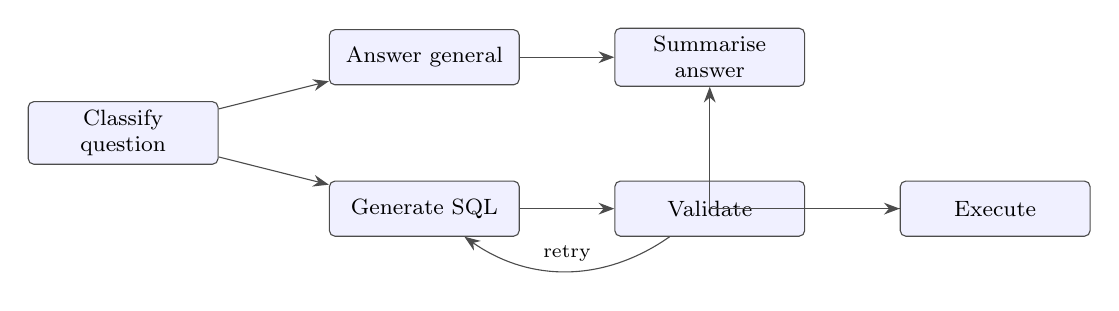
\begin{tikzpicture}[node distance=7mm and 12mm]
  \node[gnode] (cls) {Classify question};
  \node[gnode, above right=2mm and 14mm of cls] (gen2) {Answer general};
  \node[gnode, below right=2mm and 14mm of cls] (gen) {Generate SQL};
  \node[gnode, right=of gen] (val) {Validate};
  \node[gnode, right=of val] (exe) {Execute};
  \node[gnode, right=12mm of gen2] (end) {Summarise answer};

  \draw[flow] (cls) -- (gen2);
  \draw[flow] (cls) -- (gen);
  \draw[flow] (gen) -- (val);
  \draw[flow] (val) -- (exe);
  \draw[flow] (gen2) -- (end);
  \draw[flow] (exe) -| (end);
  \draw[flow] (val) to[bend left=35] node[above,font=\scriptsize]{retry} (gen);
\end{tikzpicture}
\caption{The natural-language-to-SQL agent as a directed graph. The validate step can send the query back for a retry; only a safe query is executed.}
\label{fig:agent}
\end{figure}

Query generation and validation are kept strict, because the agent must never harm the database. The generated query has to be a single read-only \texttt{SELECT}. A deterministic check blocks dangerous keywords such as \texttt{DROP}, \texttt{DELETE} and \texttt{UPDATE}, and a second model pass checks that the query really matches the question. If a check fails, or if the query raises a database error, the agent gets feedback and tries again, up to a small number of retries. Once a query passes, it is run and the resulting rows are summarised back in natural language, in the same language as the question. A role-scoping rule can also restrict a doctor to their own patients, by forcing a condition on the provider identifier and rejecting any answer that does not respect it.

% !TEX root = ./main.tex

\section{Results}
\label{sec:results}

We report results on the Synthea dataset described in Section~\ref{sec:system}. After outlier removal, 21{,}995 of the 22{,}284 patients were used to fit the clustering model, and the remaining patients were kept as the separate group with label $-1$.

\subsection{Clustering}

To select a configuration we ran a benchmark over 63 feature subsets and several hyperparameter values, and we ranked the runs with a combined score that gives the most weight to the Gower silhouette. Table~\ref{tab:clusters} lists the best configuration for each number of clusters.

\begin{table}[t]
\caption{Best clustering configuration per number of clusters. The final pick is $k=4$.}
\label{tab:clusters}
\centering
\small
\begin{tabular}{@{}lccccc@{}}
\toprule
Config & $k$ & $\gamma$ & Silhouette & Gower & Davies-Bouldin \\
\midrule
\textbf{Final ($k{=}4$)} & \textbf{4} & auto & 0.132 & \textbf{0.350} & 2.51 \\
Best $k{=}5$ & 5 & 0.17 & 0.095 & 0.356 & 3.11 \\
Best $k{=}6$ & 6 & 0.17 & 0.029 & 0.313 & 2.59 \\
\bottomrule
\end{tabular}
\end{table}

We chose $k=4$. The five-cluster run has a slightly higher Gower silhouette (0.356 against 0.350), but only one of its clusters clears our stability threshold of about $0.20$, while in the four-cluster run all clusters do, with per-cluster values of $0.423$, $0.199$, $0.320$ and $0.396$. Since the clusters are later used as scopes for sequence mining, we prefer the smallest $k$ for which every cluster stays cohesive. The strongest features are the number of active conditions ($\eta^2 = 0.74$) and age ($\eta^2 = 0.66$) on the numerical side, and condition burden (Cramer's V $= 0.80$), gender ($0.70$), diabetes ($0.69$) and heart disease ($0.66$) on the categorical side.

Figures~\ref{fig:heatmap},~\ref{fig:numerical} and~\ref{fig:categorical} describe the final partition. The heatmap of z-scored numerical means shows a clear morbidity gradient, from cluster~0 with younger and low-burden patients to the higher-numbered clusters with more conditions and more treatment. The numerical bars confirm that active conditions and age drive most of the separation, and the categorical panel shows how condition burden, the disease flags and gender split the four groups. Read together, the clusters correspond to four recognisable populations: young low-burden patients, women of reproductive age, hypertensive adults with polypharmacy, and a pediatric or acute group.

\begin{figure}[t]
\centering
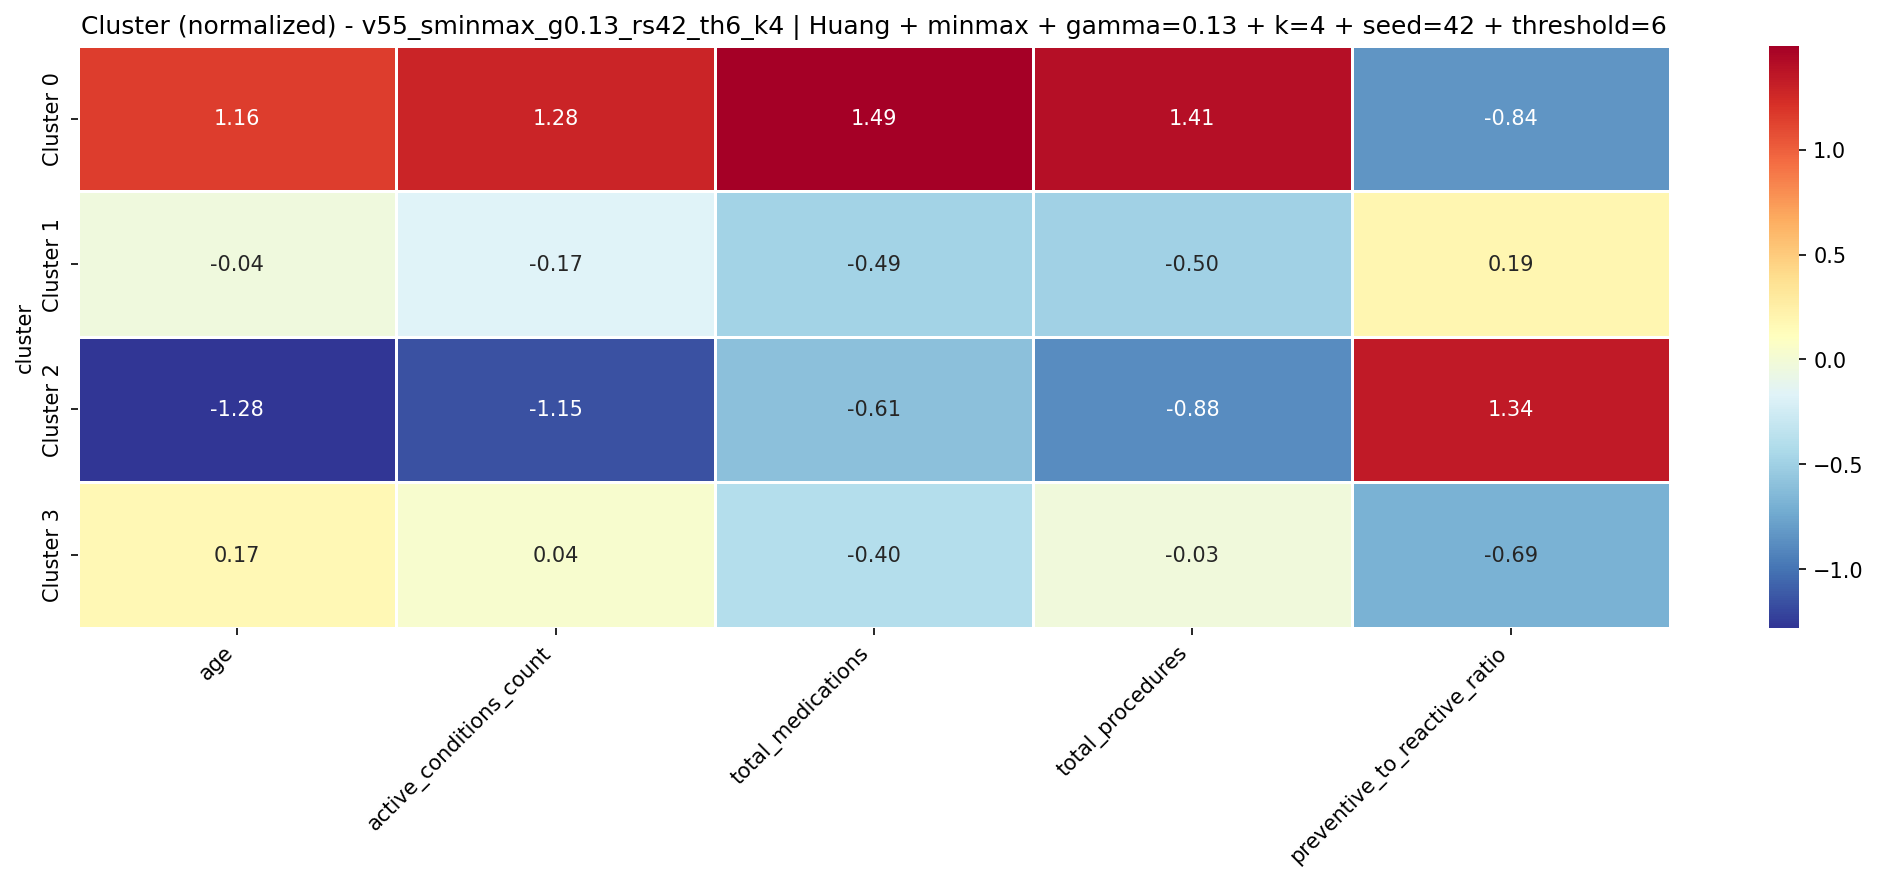
\includegraphics[width=0.92\linewidth]{figs/cluster_heatmap.png}
\caption{Z-scored numerical feature means per cluster ($k=4$). Warm colours are above the population average, cool colours below it.}
\label{fig:heatmap}
\end{figure}

\begin{figure}[t]
\centering
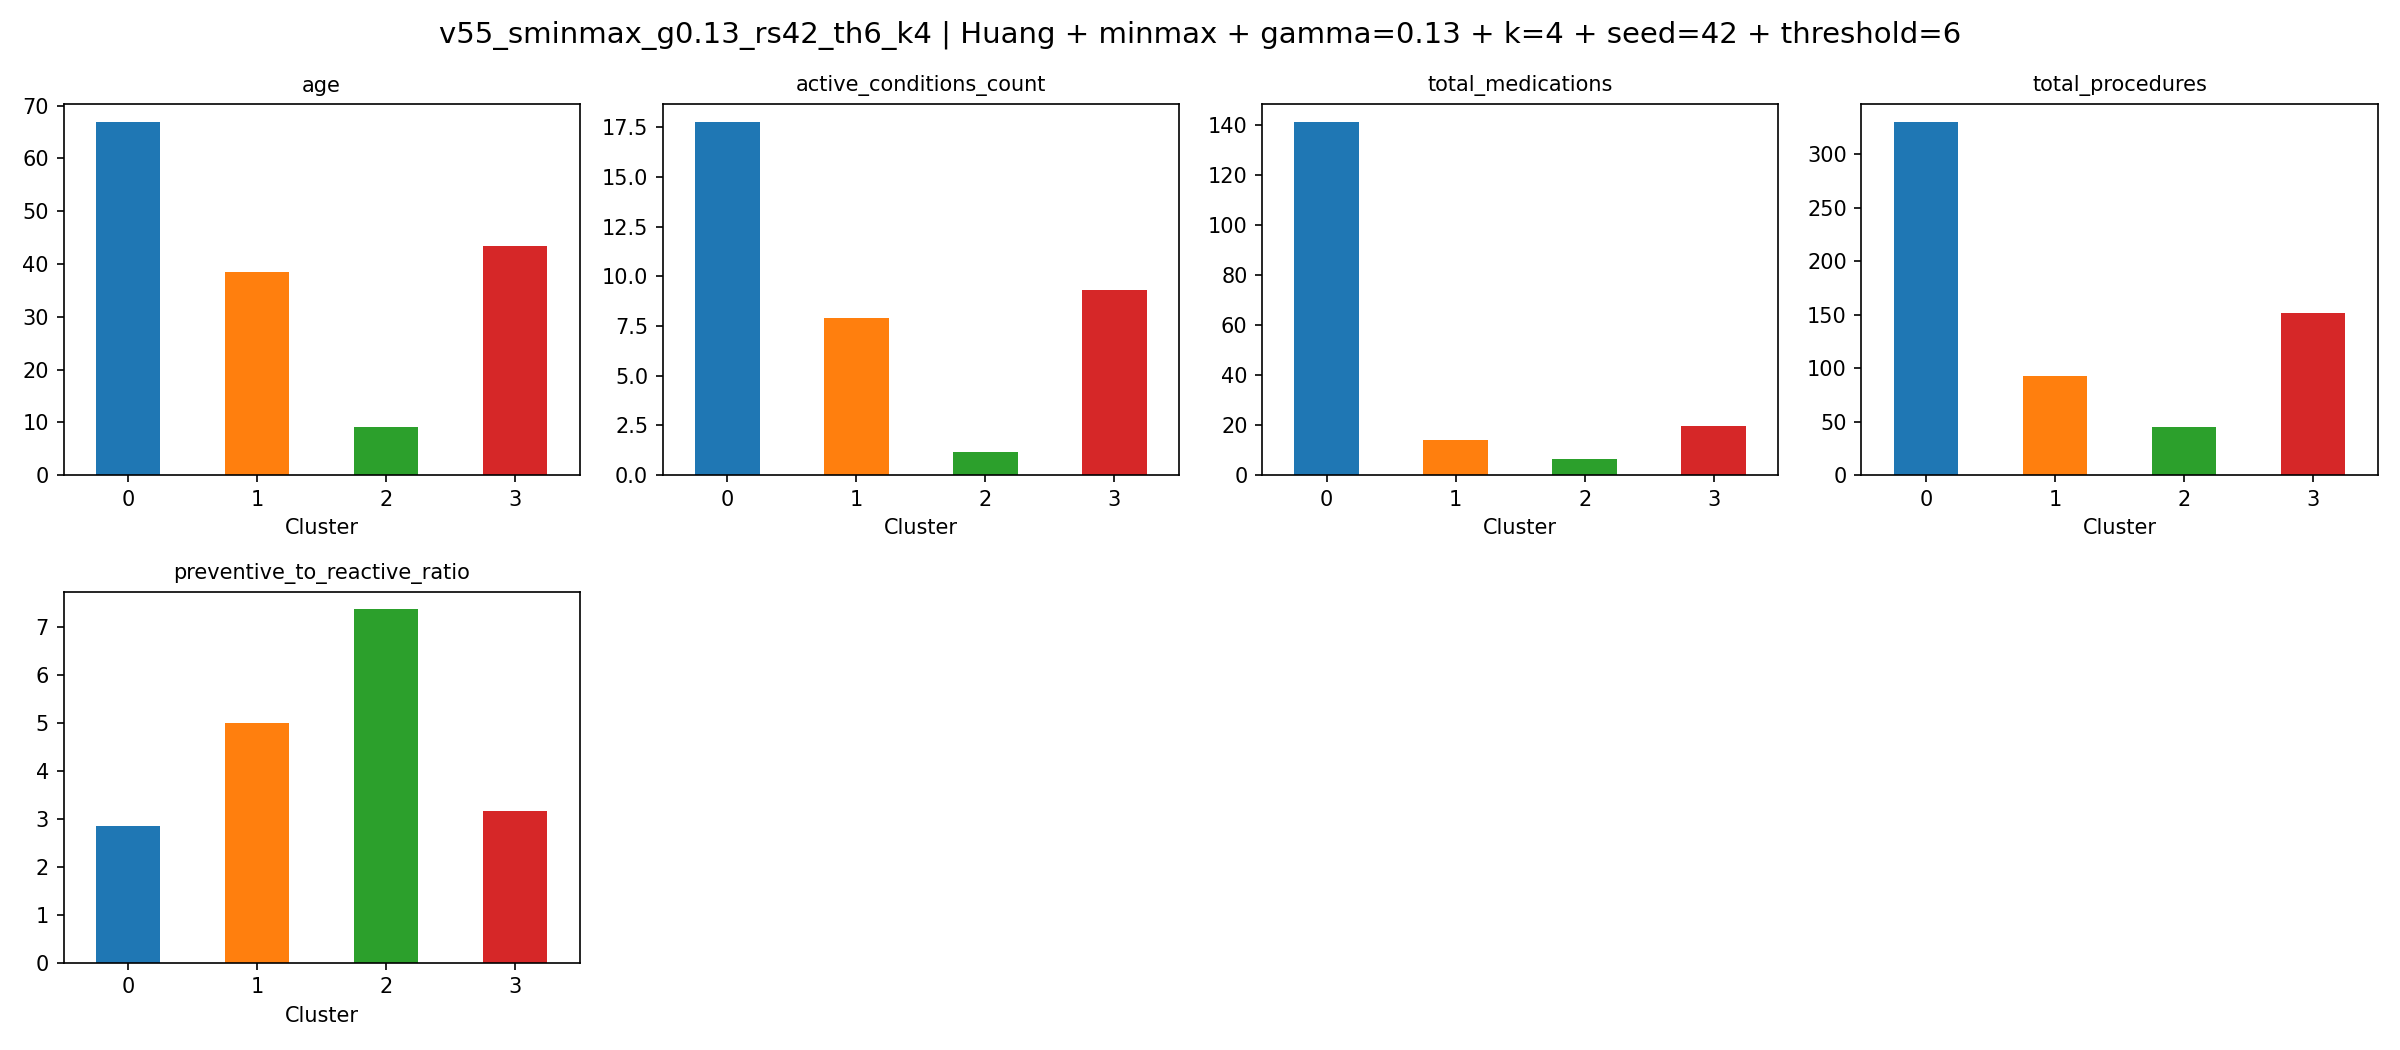
\includegraphics[width=0.92\linewidth]{figs/cluster_numerical.png}
\caption{Per-cluster means of the five numerical features.}
\label{fig:numerical}
\end{figure}

\begin{figure}[t]
\centering
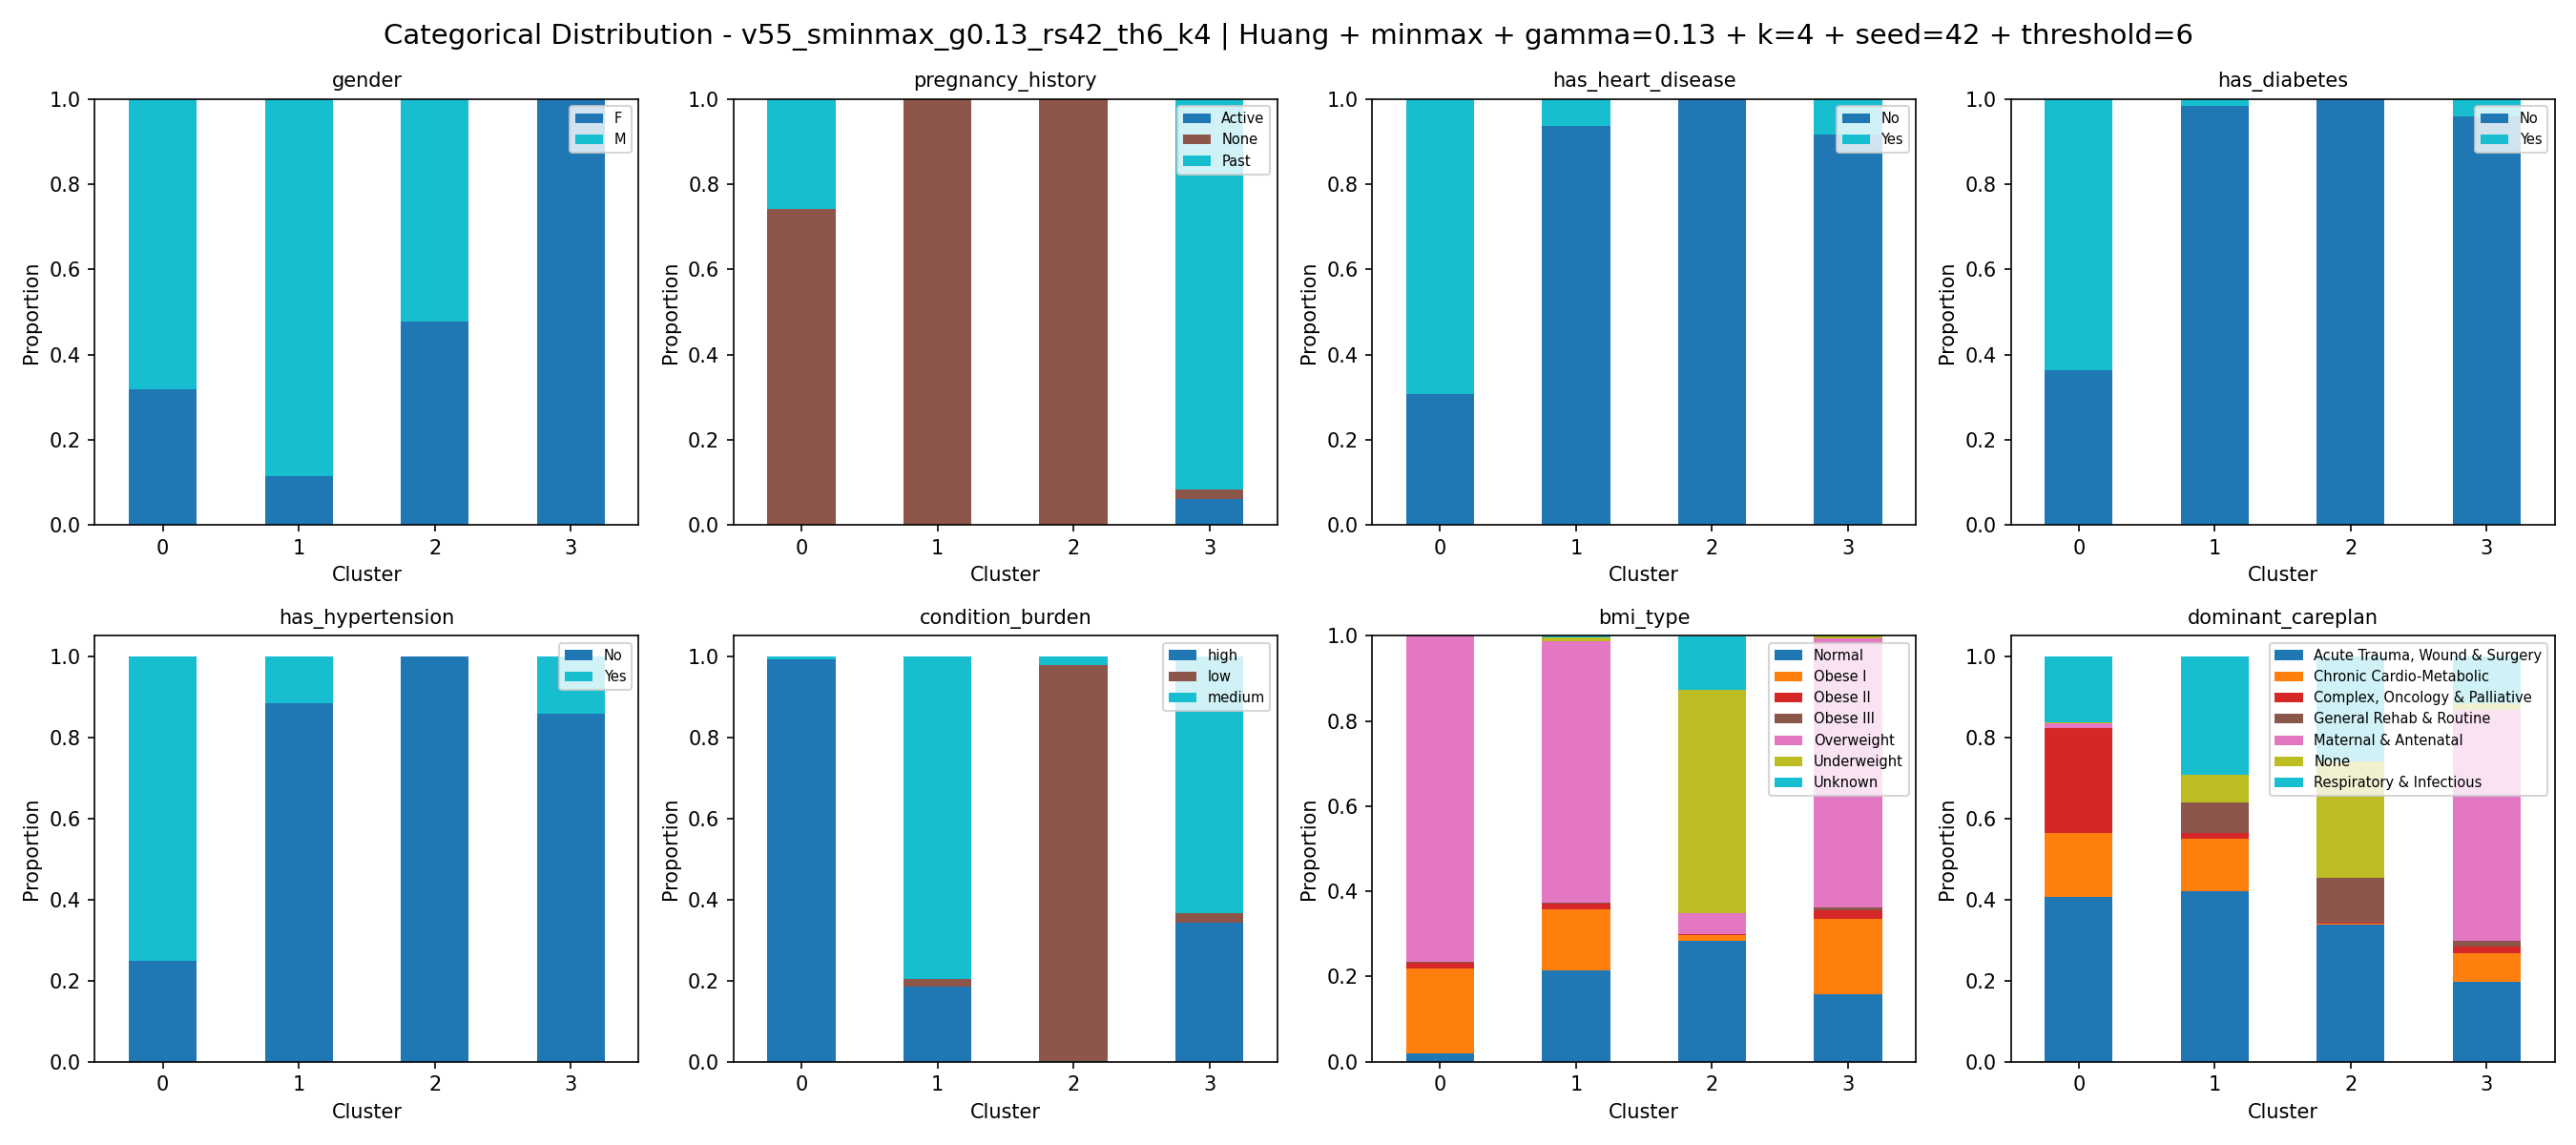
\includegraphics[width=0.92\linewidth]{figs/cluster_categorical.png}
\caption{Per-cluster proportions of the eight categorical features.}
\label{fig:categorical}
\end{figure}

\subsection{Sequence Mining}

The clearest way to show the effect of the pipeline is to compare the first and the last version of the miner on the same data. Table~\ref{tab:ablation} shows the top pattern in each case. When we rank by raw support (version v0), the best result is an administrative loop, and almost the entire top of the list is filled with near-identical dental cleaning steps that around 93\% of patients receive. After we add the GML score and the diversity selection (version v6), the top of the list becomes a set of short, clinically coherent care paths.

\begin{table}[t]
\caption{Effect of the ranking. Top pattern when ranking by support (v0) and by geometric mean lift with diversity selection (v6).}
\label{tab:ablation}
\centering
\small
\begin{tabular}{@{}p{0.08\linewidth}p{0.82\linewidth}@{}}
\toprule
Ver. & Top-ranked pattern \\
\midrule
v0 & Medication review due $\rightarrow$ Medication reconciliation $\rightarrow$ Medication review due \emph{(support 96\%, no clinical value)} \\[2pt]
v6 & Laceration $\rightarrow$ Wound care $\rightarrow$ Suture open wound \emph{(GML 0.97)} \\
\bottomrule
\end{tabular}
\end{table}

Mining each scope on its own produces between 175 and 252 frequent patterns. Table~\ref{tab:patterns} gives representative patterns from the hypertensive cluster and from the outlier scope. The hypertensive cluster is dominated by chronic-disease management, for example a furosemide and oxygen sequence for fluid overload, a dialysis and epoetin loop, and an antihypertensive drug paired with screening procedures. The outlier scope is the most striking result. Because we mine the label $-1$ group separately, high-cost pathways become visible: chemotherapy with cisplatin followed by hospice care, kidney transplantation with tacrolimus, and a recurring heart-failure sequence. These pathways are below the global support floor and would be invisible if we mined the whole cohort at once.

\begin{table}[t]
\caption{Representative mined pathways from two scopes (ranked by GML).}
\label{tab:patterns}
\centering
\small
\begin{tabular}{@{}p{0.16\linewidth}p{0.66\linewidth}r@{}}
\toprule
Scope & Pattern & GML \\
\midrule
Cluster 2 & Furosemide $\rightarrow$ Oxygen by mask $\rightarrow$ Prone position $\rightarrow$ Furosemide & 0.89 \\
Cluster 2 & Epoetin Alfa $\rightarrow$ Renal dialysis $\rightarrow$ Epoetin Alfa & 0.81 \\
Cluster 2 & Lisinopril $\rightarrow$ Depression screening $\rightarrow$ Substance-use assessment & 0.41 \\
Outliers ($-1$) & Chemotherapy + radiation $\rightarrow$ Cisplatin $\rightarrow$ Hospice care & 0.85 \\
Outliers ($-1$) & Renal review $\rightarrow$ Tacrolimus $\rightarrow$ Kidney transplantation & 0.90 \\
\bottomrule
\end{tabular}
\end{table}

Taken together, the results show that the four-cluster partition is not only defensible by its metrics but also meaningful in content. Each cluster's top patterns describe a clearly different care population, which is exactly the property we need for cluster-scoped analysis in the dashboard.

% !TEX root = ./main.tex

\section{Discussion and Conclusion}
\label{sec:conclusion}

We presented HospitAI, a platform that joins three analytics steps over hospital data: mixed-data patient clustering, clinical sequence mining and AI-generated interpretation. The clustering produces a small number of readable patient groups. The sequence mining, with its geometric mean lift ranking and its diversity selection, returns care paths that are clinically meaningful rather than just frequent. The language layer turns the numbers into short summaries and lets users ask questions in plain language.

The design has clear strengths. The cluster-then-mine approach keeps each result local to a patient group, which makes the patterns easier to read and to compare. Treating outliers as their own scope is a simple idea that pays off, because it brings rare but high-cost pathways such as oncology, dialysis and heart failure back into view, instead of letting them fall below the global support floor. The verbaliser design, where the model only describes precomputed numbers, is a practical way to use an LLM in a clinical setting without letting it invent facts.

There are also honest limitations. The data is synthetic, so the patterns reflect how Synthea models care and not the behaviour of a real hospital. We did not run a formal clinical validation with physicians, and the quality of the mined patterns was judged mostly by inspection rather than by a numeric benchmark against other mining algorithms. The platform depends on a single external LLM, which raises questions of cost, reproducibility and data governance that a hospital would have to solve before real use. One of the cleaning filters is tuned to the dataset, so part of the preprocessing is dataset-specific and would need to be revisited on new data.

Future work follows from these points. The first step is to test the pipeline on a real, de-identified dataset and to ask clinicians to rate the mined pathways. A second step is to add a proper evaluation of the sequence patterns, for example by comparing them with clinical guidelines or with other miners such as those reviewed in the surveys we cited. A third step is to study the language layer in more detail, including the accuracy of the SQL agent and the faithfulness of the generated summaries. We would also like to replace the dataset-specific filter with a more general rule, so the pipeline transfers more easily to other hospitals.

Overall, the project shows that standard algorithms become much more useful when they are wrapped in careful preprocessing, a task-aware ranking and a readable output layer. For a hospital that already stores its data, this kind of platform could be a low-cost way to begin understanding its own patient population.


\subsubsection*{Conflict of Interest.}
The author declares that there is no conflict of interest.

\subsubsection*{Statement of Informed Consent.}
This study did not involve human participants. All experiments were carried out on synthetic patient data generated with Synthea, so informed consent was not required.

\subsubsection*{Human and Animal Rights.}
This article does not contain any studies with human participants or animals performed by the author. No real patient data was used.

\bibliographystyle{splncs04}
\bibliography{references}

\end{document}
